\documentclass{article}
\usepackage[utf8]{inputenc}
\usepackage{hyperref}
\usepackage{graphicx}

\title{\textbf{Elaboration 1: Planning}}
\author{Emily Hunt}
\date{August 2019}

\begin{document}

\maketitle

View in Overleaf: \url{https://www.overleaf.com/read/ncsqngkgzrgs}

\section*{Instructions}
Using the step-by-step breakdown of your problems / solutions developed last week, identify technologies (programming languages, software libraries, APIs (Application programming interfaces, the means by which one program talks to another program) and other components of a modern data collection or processing workflow) that could accomplish each step. You may want to specify more than one possible technology. 

\section*{Scoping II Decomposition}
I realised I partially misunderstood the expectation for decomposition last week (my response for this section was more appropriate for the algorithm section). So I will first re-attempt decomposition, by breaking down my usual process for analysing the colour of films.

\begin{enumerate}
    \item I watch a film in its entirety taking notes on the colour palette used and how various colours are used thematically. These will most likely \textbf{not} be labelled very clearly (e.g. with time stamps) but just be general notes.
    \item When reviewing these notes to write an essay etc., I will have to go back through the film and try and work out which part of it the notes are referencing, which can be a very time consuming and fiddly process.
\end{enumerate} 

Using the XY Problem resource (\url{http://xyproblem.info/}), I also realised that my issue was not solely analysing the colour of films, but organising my notes concerning these. Therefore, the technologies listed below to accomplish each step in the decomposition will be divided into those that assist with colour analysis, and note taking. These will be evaluated in terms of what Brian noted on Slack to be signs of a good tool (well written and easily understandable documentation, as well as recent maintenance (indicating wide use)).

\section*{Solutions for Colour Analysis}
I couldn't really find a tool that did specifically what I identified in scoping (measures the number of times a colour appears throughout a film), so I switched my focus to tools that would create a colour map of a film.

\subsection{GitHub: Cinemetrics (Original)}
URL: \url{https://github.com/freder/cinemetrics}\\
This tool would be ideal, as in addition to producing a map of the colours present in a film, it provides a representation of a number of the film's other features, such as shot duration and motion, which are things I hadn't really considered before. However, this tool will probably not be viable to use, as it fails to meed a number of the criteria identified on Slack: 
\begin{itemize}
    \item Documentation: There is no documentation provided with this tool, as explicitly noted on its GitHub repository.
    \item Maintenance: The last commits for this project were 8/9 years ago.
\end{itemize}

\subsection{GitHub: Cinemetrics}
URL: \url{https://github.com/suite22/cinemetrics}\\
This tool is a different version of the previously identified one. It seems more feasible than the other option in one respect:

\begin{itemize}
    \item Documentation: Detailed documentation is provided with this tool. From a preliminary reading, it seems to be understandable.
    \item Maintenance: However, similarly to the aforementioned tool, a number of the latest commits for a number of the files were 8 years ago, though a few were as recent as 3/4 years ago.
\end{itemize}
I did an initial test of this software. I installed vagrant as instructed, downloaded a zip of the repository and then in Terminal, made the copy of the repository the working directory and entered 'vagrant up'. This produced a message informing me I needed to install a 'provider', with VirtualBox recommended. However, I had some issues with security and privacy settings when trying to install VirtualBox, so stopped the test here.

\subsection{GitHub: Colors-of-Film}
URL: \url{https://github.com/sacert/Colors-of-Film}\\
This tool may also prove to be a viable option. It allows customisation of the size (length/width) of the output colour map image.
\begin{itemize}
    \item Documentation: The documentation is very straightforward and clear, and it seems the software is simple to use.
    \item Maintenance: The last commits were 2/3 years ago, and the repository has 16 stars.
\end{itemize}

\subsection{GitHub: FilmStrip}
URL: \url{https://github.com/ArkadiusBear/FilmStrip}\\
The tool may also be viable for producing a colour map of a film. At allows the customisation of a number of aspects of the output image, including size, ratio and density.

\begin{itemize}
    \item Documentation: Really clear documentation is provided regarding what the tool does and how it works, though there doesn't appear to be much documentation in relation to how to use the tool.
    \item Maintenance: The last commits were 8 months ago, making this the most recently updated repository of all the tools listed. However, these commits were only over two days, indicating there has not been a long process of testing and updating.
\end{itemize}
 
\section*{Solutions for Note Taking}
URL: \url{http://www.clipnotes.org/}\\
Though I can't locate the code for this tool, it seems like it could be a really valuable tool. It appears that for it to work, you download the app, have a film file and your notes (with a time stamp) in an XML file. You can then open the film file and notes in the app, and it will display the notes at the appropriate time in the film.
\begin{itemize}
    \item Documentation: There is really detailed documentation on how to use the software on the website, as well as a trouble shooting section.
    \item Maintenance: From what I can see, the last update of the software was 2015.
\end{itemize}

This solution could be potentially combined with one of the colour analysis solutions, so that a specific portion of the colour map could be linked (through the XML file?) to that specific section of the film if I want to view it in more detail.

\subsection*{Inspiration}

The inspiration for the potential combination for these two tools came from an app called 'Animated' by Walt Disney Animation Studios. It includes a colour map of each of the studio's films which you can select and scrub through to see certain stills (\autoref{fig:colourmaps}). While this is useful to me in its current form (as I plan to analyse Disney films in my thesis) the production of colour maps is something I would like to learn how to do for potential future studies. Furthermore, in their current form the colour maps in this app are difficult to navigate as it is really fiddly to select and scrub through a specific film. I would like to be able to have a colour map and go that section of the film to look at in more detail, while also being able to see the notes I have written, which is what I am proposing in this elaboration.

\begin{figure}[htp]
    \centering
    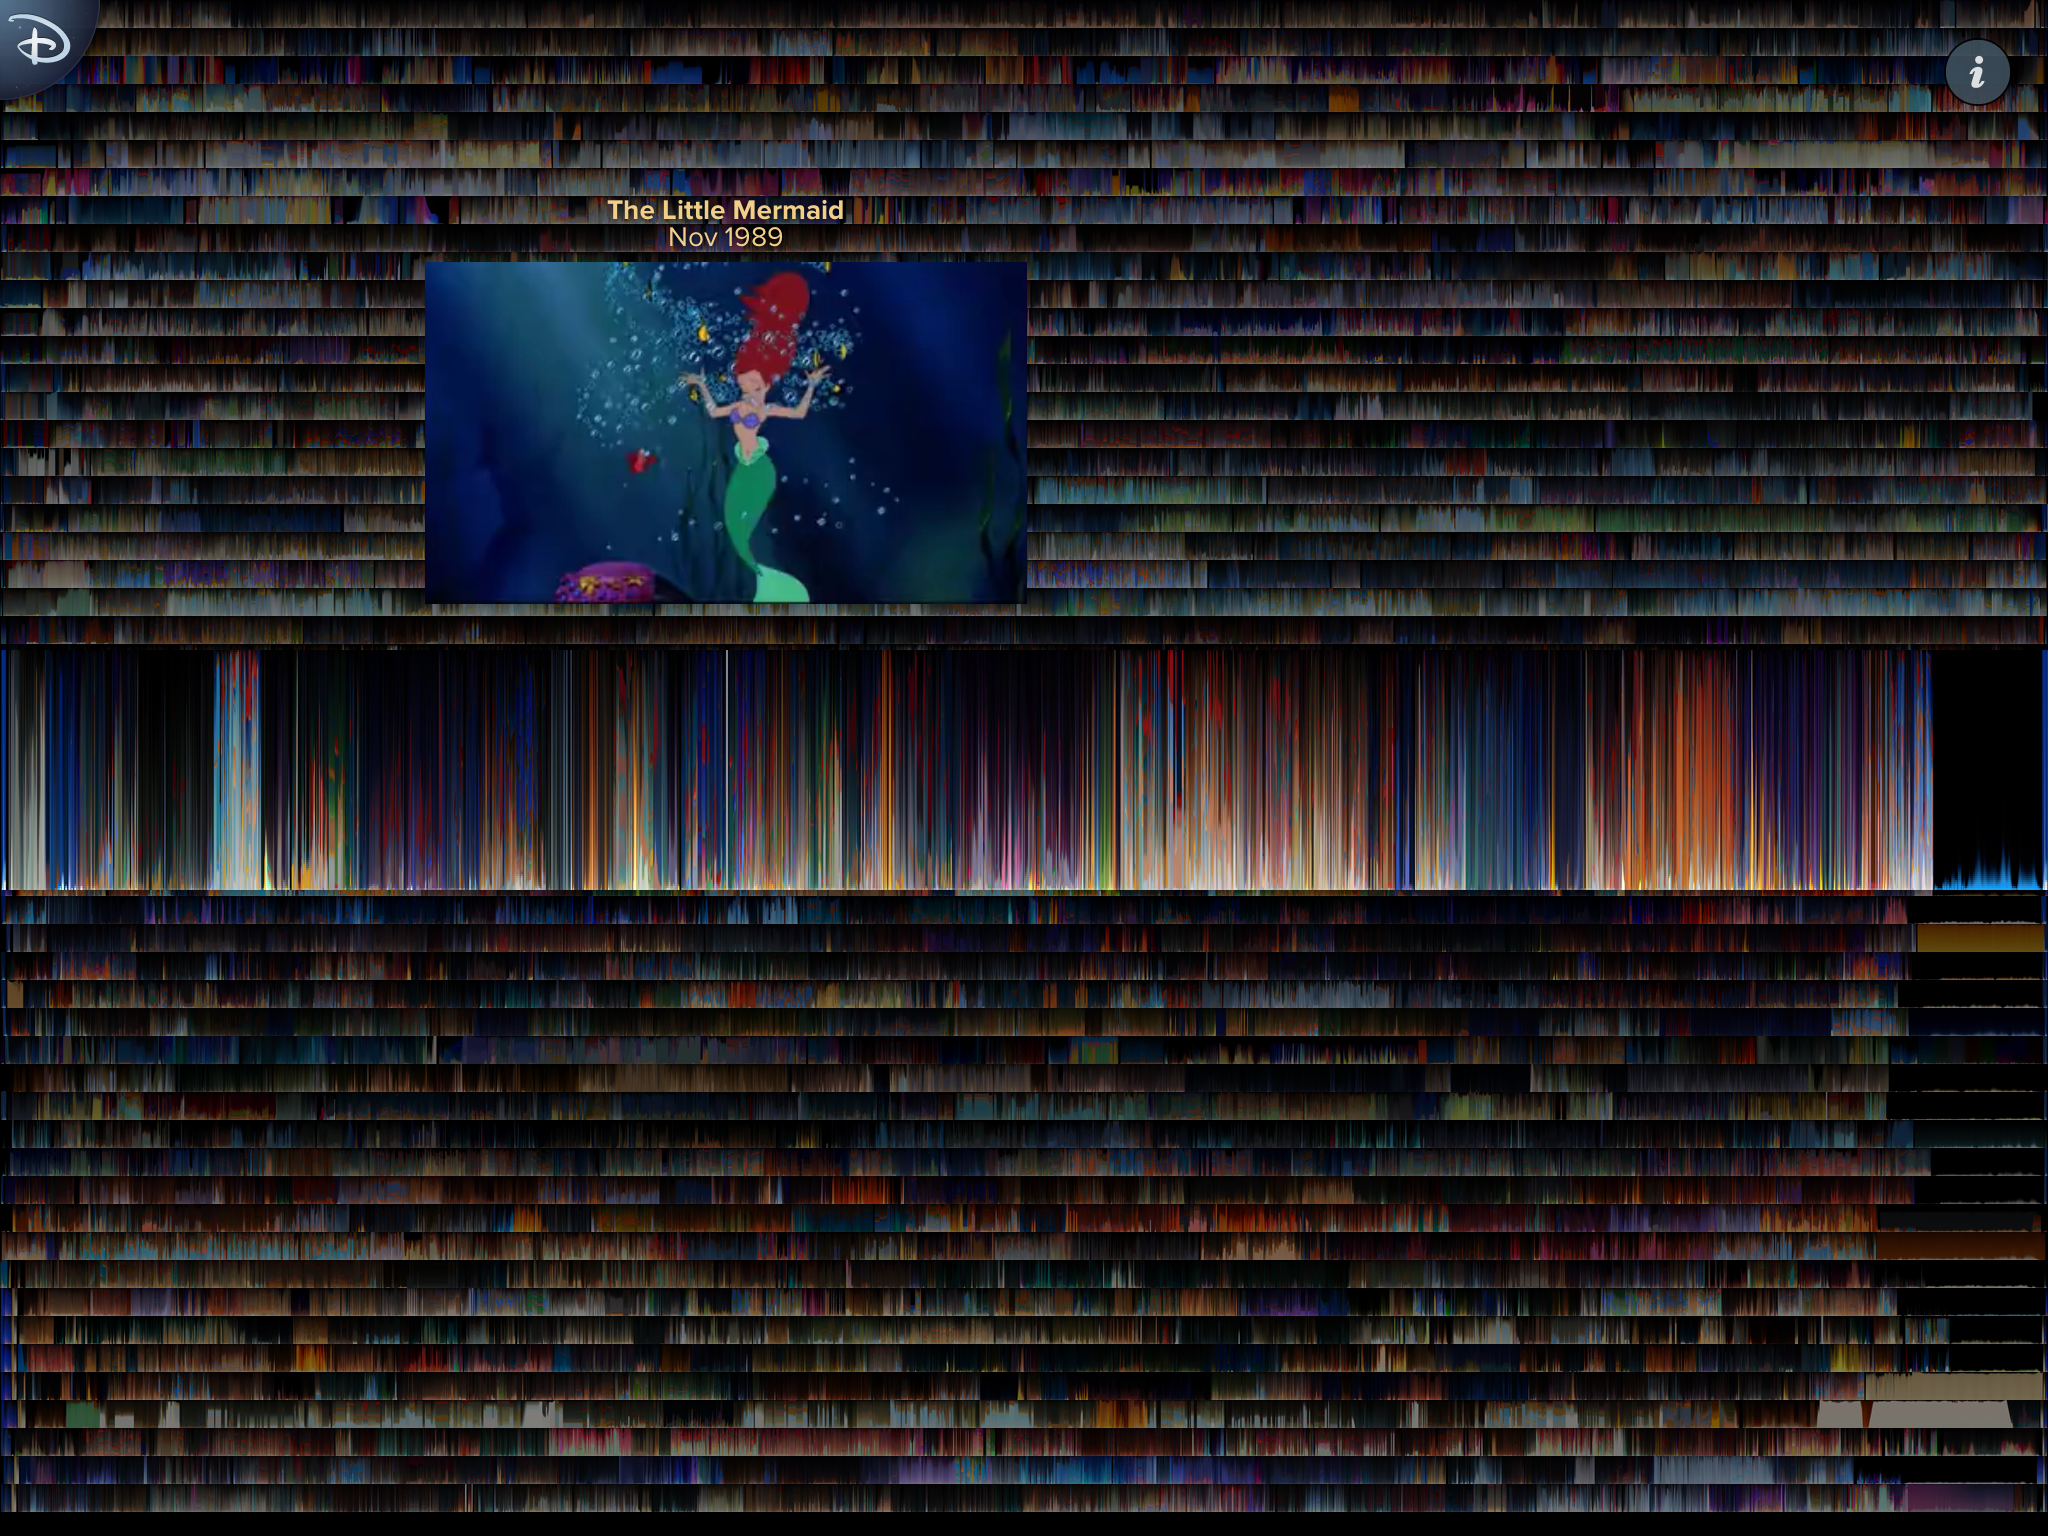
\includegraphics[width=12cm]{IMG_9495.PNG}
    \caption{Colour Maps of Disney Films in the 'Animated' App}
    \label{fig:colourmaps}
\end{figure}

\end{document}
